% !TeX program = XeLaTeX or LuaLaTeX
% !TeX encoding = UTF-8 Unicode
\documentclass[a4paper,oneside,12pt]{article}
%%%%%%%%%%%%%%%%%%%%%%%%%%%%%%%%%%%%%%%%%%%%%%%%%%%%%%%%%%%%%%%%%%%%%%%%%%%%%%%%%
%% Packages
%%%%%%%%%%%%%%%%%%%%%%%%%%%%%%%%%%%%%%%%%%%%%%%%%%%%%%%%%%%%%%%%%%%%%%%%%%%%%%%%%
\usepackage[spanish]{babel}
\usepackage{multirow}
\usepackage{amsmath}
\usepackage{fontspec}
\usepackage[xetex]{graphicx}
\usepackage{csquotes}
\usepackage{a4wide} %%Smaller margins, more text per page.
\usepackage{longtable} %%For tables that exceed a page width
\usepackage{pdflscape} %%Adds PDF sup­port to the land­scape en­vi­ron­ment of pack­age
\usepackage{caption} %%Pro­vides many ways to cus­tomise the cap­tions in float­ing en­vi­ron­ments like fig­ure and ta­ble
\usepackage{float} %%Im­proves the in­ter­face for defin­ing float­ing ob­jects such as fig­ures and ta­bles
\usepackage[tablegrid,nochapter]{vhistory} %%Vhis­tory sim­pli­fies the cre­ation of a his­tory of ver­sions of a doc­u­ment
\usepackage[nottoc]{tocbibind} %%Au­to­mat­i­cally adds the bib­li­og­ra­phy and/or the in­dex and/or the con­tents, etc., to the Ta­ble of Con­tents list­ing
\usepackage[toc,page]{appendix} %%The ap­pendix pack­age pro­vides var­i­ous ways of for­mat­ting the ti­tles of ap­pen­dices
\usepackage{pdfpages} %%This pack­age sim­pli­fies the in­clu­sion of ex­ter­nal multi-page PDF doc­u­ments in LATEX doc­u­ments
\usepackage[rightcaption]{sidecap} %%De­fines en­vi­ron­ments called SC­fig­ure and SCtable (anal­o­gous to fig­ure and ta­ble) to type­set cap­tions side­ways
% \usepackage{cite} %%The pack­age sup­ports com­pressed, sorted lists of nu­mer­i­cal ci­ta­tions, and also deals with var­i­ous punc­tu­a­tion and other is­sues of rep­re­sen­ta­tion, in­clud­ing com­pre­hen­sive man­age­ment of break points
\usepackage[printonlyused]{acronym} %%This pack­age en­sures that all acronyms used in the text are spelled out in full at least once. It also pro­vides an en­vi­ron­ment to build a list of acronyms used
% \usepackage[pdftex,scale={.8,.8}]{geometry} %%The pack­age pro­vides an easy and flex­i­ble user in­ter­face to cus­tomize page lay­out, im­ple­ment­ing auto-cen­ter­ing and auto-bal­anc­ing mech­a­nisms so that the users have only to give the least de­scrip­tion for the page lay­out. For ex­am­ple, if you want to set each mar­gin 2cm with­out header space, what you need is just \usep­a­ck­age[mar­gin=2cm,no­head]{ge­om­e­try}.
\usepackage{layout} %%The pack­age de­fines a com­mand \lay­out, which will show a sum­mary of the lay­out of the cur­rent doc­u­ment
\usepackage{subfigure} %%Pro­vides sup­port for the ma­nip­u­la­tion and ref­er­ence of small or ‘sub’ fig­ures and ta­bles within a sin­gle fig­ure or ta­ble en­vi­ron­ment.
\usepackage[toc]{glossaries} %%The glos­saries pack­age sup­ports acronyms and mul­ti­ple glos­saries, and has pro­vi­sion for op­er­a­tion in sev­eral lan­guages (us­ing the fa­cil­i­ties of ei­ther ba­bel or poly­glos­sia).
\usepackage[left,pagewise,modulo]{lineno} %%Adds line num­bers to se­lected para­graphs with ref­er­ence pos­si­ble through the LATEX \ref and \pageref cross ref­er­ence mech­a­nism
\usepackage[xetex,colorlinks=false,hidelinks,pdfstartview=FitV,bookmarks=true]{hyperref}%%The hy­per­ref pack­age is used to han­dle cross-ref­er­enc­ing com­mands in LATEX to pro­duce hy­per­text links in the doc­u­ment. 
\usepackage{metainfo}
\usepackage[top=1in,bottom=1in,left=1in,right=1in]{geometry}
% \usepackage[a4paper,left=2.5cm,right=2.5cm,top=\dimexpr15mm+1.5\baselineskip,bottom=2cm]{geometry}
\usepackage{geometry}
% \usepackage[pagestyles,raggedright]{titlesec}
\usepackage{etoolbox}
\usepackage{tabularx}
\usepackage{ltxtable}
\usepackage[style=ieee]{biblatex}
\bibliography{base/Docker.bib}
\usepackage[nottoc]{tocbibind}
\usepackage[official]{eurosym}
\usepackage{gensymb}
\usepackage{qrcode}
\usepackage{numprint}
\usepackage{mathtools}
\usepackage[nice]{nicefrac}
\usepackage{tikz}
\usetikzlibrary{arrows,automata,babel,positioning,calc}
\usepackage{%
    array, %%An ex­tended im­ple­men­ta­tion of the ar­ray and tab­u­lar en­vi­ron­ments which ex­tends the op­tions for col­umn for­mats, and pro­vides "pro­grammable" for­mat spec­i­fi­ca­tions
    booktabs, %%The pack­age en­hances the qual­ity of ta­bles in LATEX, pro­vid­ing ex­tra com­mands as well as be­hind-the-scenes op­ti­mi­sa­tion
    dcolumn, %%
    rotating,
    shortvrb,
    units,
    url,
    longtable,
    lscape,
    qtree,
    skmath,	
    enumitem,
    wasysym,
    mathcomp,
    titling,
    libertine,
    fancyhdr,
}

% Necessary packages for the titlepage:
\usepackage{comment}

\newcommand{\bigO}[1]{%
  \text{\usefont{OMS}{cmsy}{m}{n}O}\left(#1\right)%
}
%%%%%%%%%%%%%%%%%%%%%%%%%%%%%%%%%%%%%%%%%%%%%%%%%%%%%%%%%%%%%%%%%%%%%%%%%%%%%%%%%
%% Java --> latex 
%%%%%%%%%%%%%%%%%%%%%%%%%%%%%%%%%%%%%%%%%%%%%%%%%%%%%%%%%%%%%%%%%%%%%%%%%%%%%%%%%
\setmonofont{Fira Code}[
  Contextuals=Alternate,
  Ligatures = {Common,Rare}
]
\usepackage{letltxmacro}
\LetLtxMacro\oldttfamily\ttfamily
\DeclareRobustCommand{\ttfamily}{\oldttfamily\csname ttsize\endcsname}
\newcommand{\settttsize}[1]{\def\ttsize{#1}}%
\usepackage{lstfiracode}
\usepackage{listings}

\lstset{ %
  backgroundcolor=\color{white},   % Indica el color de fondo; necesita que se añada \usepackage{color} o \usepackage{xcolor}
  basicstyle=\footnotesize\ttfamily,        % Fija el tamaño del tipo de letra utilizado para el código
  breakatwhitespace=false,         % Activarlo para que los saltos automáticos solo se apliquen en los espacios en blanco
  inputencoding=utf8,
  breaklines=true,                 % Activa el salto de línea automático
  captionpos=b,                    % Establece la posición de la leyenda del cuadro de código
  commentstyle=\color{darkgreen},    % Estilo de los comentarios
  extendedchars=true,              % Permite utilizar caracteres extendidos no-ASCII; solo funciona para codificaciones de 8-bits; para UTF-8 no funciona. En xelatex necesita estar a true para que funcione.
  frame=single,	                   % Añade un marco al código
  keepspaces=true,                 % Mantiene los espacios en el texto. Es útil para mantener la indentación del código(puede necesitar columns=flexible).
  columns=flexible,
  keywordstyle=\color{darkorange},       % estilo de las palabras clave
  numbers=left,                    % Posición de los números de línea (none, left, right).
  numbersep=5pt,                   % Distancia de los números de línea al código
  numberstyle=\small\color{gray}, % Estilo para los números de línea
  rulecolor=\color{black},         % Si no se activa, el color del marco puede cambiar en los saltos de línea entre textos que sea de otro color, por ejemplo, los comentarios, que están en verde en este ejemplo
  showspaces=false,                % Si se activa, muestra los espacios con guiones bajos; sustituye a 'showstringspaces'
  showstringspaces=false,          % subraya solamente los espacios que estén en una cadena de esto
  showtabs=false,                  % muestra las tabulaciones que existan en cadenas de texto con guión bajo
  stringstyle=\color{darkgreen},     % Estilo de las cadenas de texto
  style=FiraCodeStyle,
  identifierstyle=\color{blue},
  tabsize=4,	                   % Establece el salto de las tabulaciones a 2 espacios
  title=\lstname,                   % muestra el nombre de los ficheros incluidos al utilizar
  caption=\lstname,
  literate={á}{{\'a}}1 {é}{{\'e}}1 {í}{{\'{\i}}}1 {ó}{{\'o}}1 {ú}{{\'u}}1 {Á}{{\'A}}1 {É}{{\'E}}1 {Í}{{\'I}}1 {Ó}{{\'O}}1 {Ú}{{\'U}}1 {ü}{{\"u}}1 {Ü}{{\"U}}1 {ñ}{{\~n}}1 {Ñ}{{\~N}}1 {¿}{{?``}}1 {¡}{{!``}}1 {º}{\textdegree}1,
  postbreak=\mbox{\textcolor{red}{$\hookrightarrow$}\space},
}
\lstdefinestyle{C}{%
  language=C,                 % El lenguaje del código
  otherkeywords={__attribute__, __interrupt__, inline, asm, uint8_t, uint16_t,%
  uint32_t, uint64_t, time_t, size_t, servo_t, motor_t, Nop,%
  point_t, angle_t, double64_t, int_fast64_t, bool, true, false, stdbool, stdint,%
  stdlib, stddef, NULL}           % Si se quieren añadir otras palabras clave al lenguaje
}
\lstdefinestyle{Python}{%
  language=Python
}

\lstdefinestyle{Ada}{%
  language=Ada
}
\lstdefinestyle{bash}{%
  language=bash,
  otherkeywords={sudo,chmod,chown,chgrp,ls,mkdir,touch,useradd,groupadd,usermod}
}
\lstdefinestyle{R}{%
  language=R,
  otherkeywords={0,1,2,3,4,5,6,7,8,9},
  morekeywords={TRUE,FALSE},
  deletekeywords={data,frame,length,as,character,time,ts}
}
\usepackage{xcolor}
\definecolor{pblue}{rgb}{0.13,0.13,1}
\definecolor{pgreen}{rgb}{0,0.5,0}
\definecolor{pred}{rgb}{0.9,0,0}
\definecolor{pgrey}{rgb}{0.46,0.45,0.48}
\definecolor{darkgreen}{rgb}{0.0, 0.4, 0.0}
\definecolor{darkorange}{rgb}{1.0, 0.55, 0.0}
% \usepackage{inconsolata}
%%%%%%%%%%%%%%%%%%%%%%%%%%%%%%%%%%%%%%%%%%%%%%%%%%%%%%%%%%%%%%%%%%%%%%%%%%%%%%%%%
% \setlength{\parindent}{0pt}
\setlength{\parskip}{.5\baselineskip}
%% Checkmark symbols
\usepackage{pifont}
\newcommand{\cmark}{\ding{51}}%
\newcommand{\xmark}{\ding{55}}%
\newcommand{\done}{\rlap{$\square$}{\raisebox{2pt}{\large\hspace{1pt}\cmark}}%
\hspace{-2.5pt}}
\newcommand{\wontfix}{\rlap{$\square$}{\large\hspace{1pt}\xmark}}
%%%%%%%%%%%%%%%%%%%%%%%%%%%%%%%%%%%%%%%%%%%%%%%%%%%%%%%%%%%%%%%%%%%%%%%%%%%%%%%%%
%% Creation of the header
%%%%%%%%%%%%%%%%%%%%%%%%%%%%%%%%%%%%%%%%%%%%%%%%%%%%%%%%%%%%%%%%%%%%%%%%%%%%%%%%%
\patchcmd{\chapter}{plain}{short}{}{} %$ <-- the header on chapter 1
\addto\captionsspanish{%
  \renewcommand\appendixname{Anexo}
  \renewcommand\appendixpagename{Anexos}
}
\newcolumntype{s}{>{\hsize=.5\hsize\linewidth=\hsize}X}
\newcolumntype{b}{>{\hsize=.75\hsize}X}
\newcommand{\heading}[1]{\multicolumn{1}{c}{#1}}
\newcolumntype{L}[1]{>{\hsize=#1\hsize\raggedright\arraybackslash}X}%
\newcolumntype{R}[1]{>{\hsize=#1\hsize\raggedleft\arraybackslash}X}%
\newcolumntype{C}[1]{>{\hsize=#1\hsize\centering\arraybackslash}X}%

\DeclareMathOperator{\atantwo}{atan2}

\DeclareMathOperator{\arctantwo}{arctan2}
%%%%%%%%%%%%%%%%%%%%%%%%%%%%%%%%%%%%%%%%%%%%%%%%%%%%%%%%%%%%%%%%%%%%%%%%%%%%%%%%%
%% DOCUMENT
%%%%%%%%%%%%%%%%%%%%%%%%%%%%%%%%%%%%%%%%%%%%%%%%%%%%%%%%%%%%%%%%%%%%%%%%%%%%%%%%%
\author{Javier Alonso Silva}
\title{Análisis de contenedores Docker}
\date{2021}
\pagestyle{fancy}
\fancyhf{}
\fancyhfoffset[L]{1cm} % left extra length
\fancyhfoffset[R]{1cm} % right extra length
\rhead{2021}
\chead{\thetitle}
\lhead{\slshape\nouppercase{\leftmark}}
\cfoot{\thepage}
\pagenumbering{roman}

\begin{document}

\settttsize{\footnotesize}
\ActivateVerbatimLigatures
% To add this template to the main.tex file, just add the command "\include{titlePageSLU} after "\begin{docuemnt}" in the main.tex file


% In this segment, enter the desired data to be shown at the title page
\newcommand{\thesisAuthor}{\theauthor}
\newcommand{\thesisTitle}{\thetitle}
\newcommand{\thesisSubTitle}{y sus implicaciones de seguridad}
\newcommand{\thesisTitleTranslated}{Translated Headline}
\newcommand{\thesisDegree}{Seguridad en Sistemas y Redes}
\newcommand{\university}{Universidad Politécnica de Madrid}
\newcommand{\thesisPlaceDate}{\thedate}

%------------------------------------------------------------------------------
\begin{titlepage}
\thispagestyle{empty}

% Use this line of code if both SLU loggo and company/other institution loggo is desired. The positions are possible to change with the \hspace and \vspace syntax.
\begin{figure} [H]
\vspace{-2cm}
 \centering
\begin{minipage}[t]{.45\linewidth}
  \raggedright
  % Upload and include SLU loggo here:
  \hspace*{-2cm}
\includegraphics[width=\linewidth]{upmlogo.png}
  
\end{minipage}%
  \begin{minipage}[t]{.45\linewidth}
  \vspace{-3.3cm}
 \raggedleft
% Upload and include other loggo here (loggo of wikipedia is used as an example):
 \hspace*{1cm}
\includegraphics[width =0.5\textwidth]{dockerlogo.png} \hspace*{-1cm}
 
\end{minipage}
\end{figure}


% If only the logo for SLU is desired, delete "\begin{comment}" and "\end{comment}" to use this line of code:
\begin{comment}
\begin{figure}
\vspace{-3cm}
    \hspace*{-2cm}\includegraphics[width = 0.3\textwidth]{slu_logo_webb.png}\hspace*{-2cm}
\end{figure}
\end{comment}


% Adds background picture. Delete code if no background picture is wanted.
\begin{tikzpicture}[overlay, remember picture]
\node[anchor=south west, 
      xshift=-0.2cm, 
      yshift=-0.2cm] 
     at (current page.south west)
     {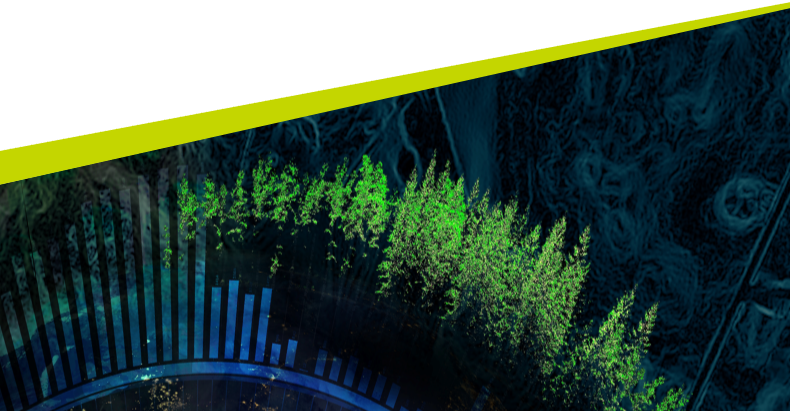
\includegraphics[width = 1.8\textwidth, height = 9cm]{background.png}}; 
\end{tikzpicture}


\vspace{1cm}
\par
\noindent
\Huge
\textbf{\thesisTitle}
\vspace{0.2cm}
\LARGE
\par
\noindent
- \thesisSubTitle\\
\rule[0.3cm]{\linewidth}{2pt}
\Large

% Delete this line if no translation is desired
% \noindent
% \textit{\thesisTitleTranslated}

\vspace{2cm}
\noindent
\LARGE
\thesisAuthor\\
\vspace{4 cm}
\small
\par \noindent
\thesisDegree
\par \noindent
\university
% \par \noindent
% \faculty
% \par \noindent
% \company
\par \noindent
\thesisPlaceDate

\end{titlepage}

\newpage
\begin{abstract}
  TO--DO
\end{abstract}

\newpage
\tableofcontents
\newpage
\pagenumbering{arabic}

\section{Introducción}
La era tecnológica ha avanzado en los últimos años a pasos agigantados, y las
demandas del sector han crecido junto a ella. No hace más de 200 años se ``descubría''
la electricidad; hace 90 años nacía la primera computadora básica capaz de realizar
operaciones aritméticas; hace 70 años nacía el transistor que sustituyó las
válvulas de vacío (figura \ref{fig:transistor}); y desde entonces, el crecimiento
ha sido exponencial \cite{HistoryTechnologyTimeline}.

\begin{figure}[H]
    \centering
    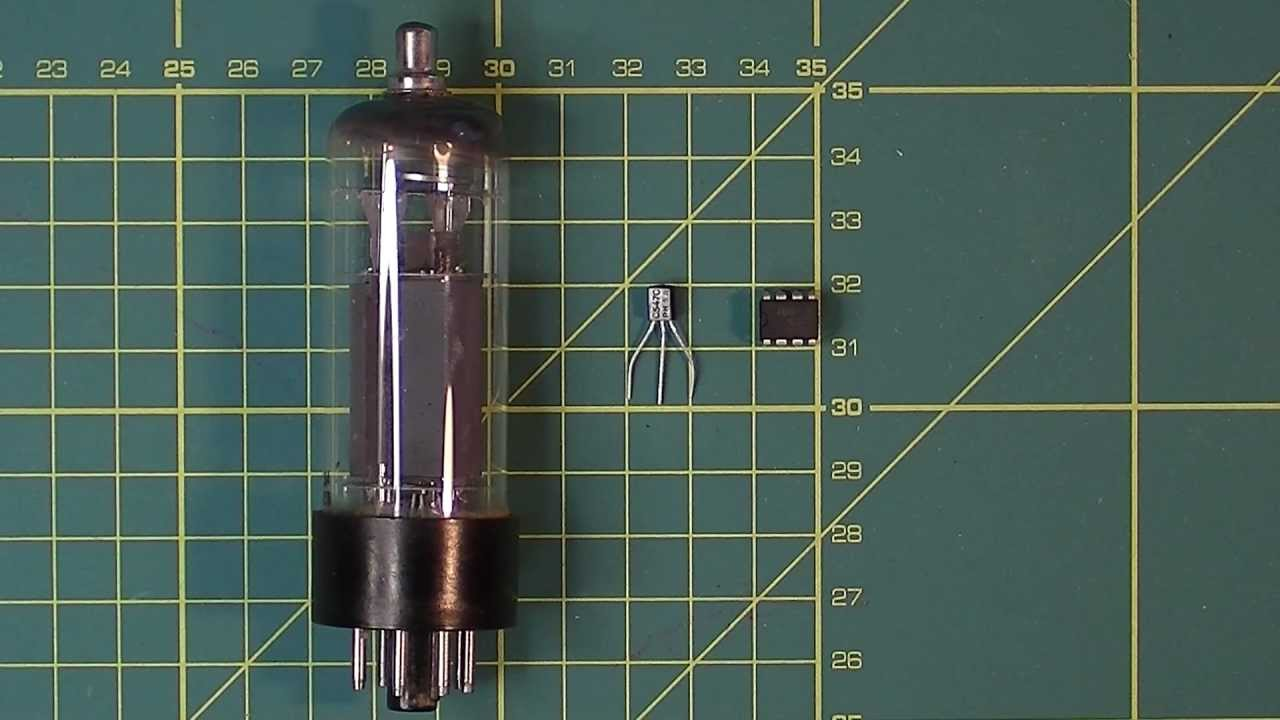
\includegraphics[width=.7\linewidth]{pictures/transistor-vs-valve.jpg}
    \caption{Comparativa de una válvula de vacío (izquierda) frente a un transistor (centro) y un circuito integrado (derecha).}
    \label{fig:transistor}
\end{figure}

Otro de los ejemplos de tecnologías que han crecido exponencialmente son los dispositivos
de almacenamiento, donde no hacía más de 20 años las capacidades máximas se estimaban
en torno a los MB (megabytes) y ahora se hablan de EB (exabytes) \cite{EvolutionDataStorage}.
Esta evolución es muy representativa también a nivel económico, ya que el coste del
almacenamiento ha ido bajando a medida pasaba el tiempo, así como el espacio físico
que ocupan los dispositivos (figura \ref{fig:disk-evolution}):

\begin{figure}[H]
    \centering
    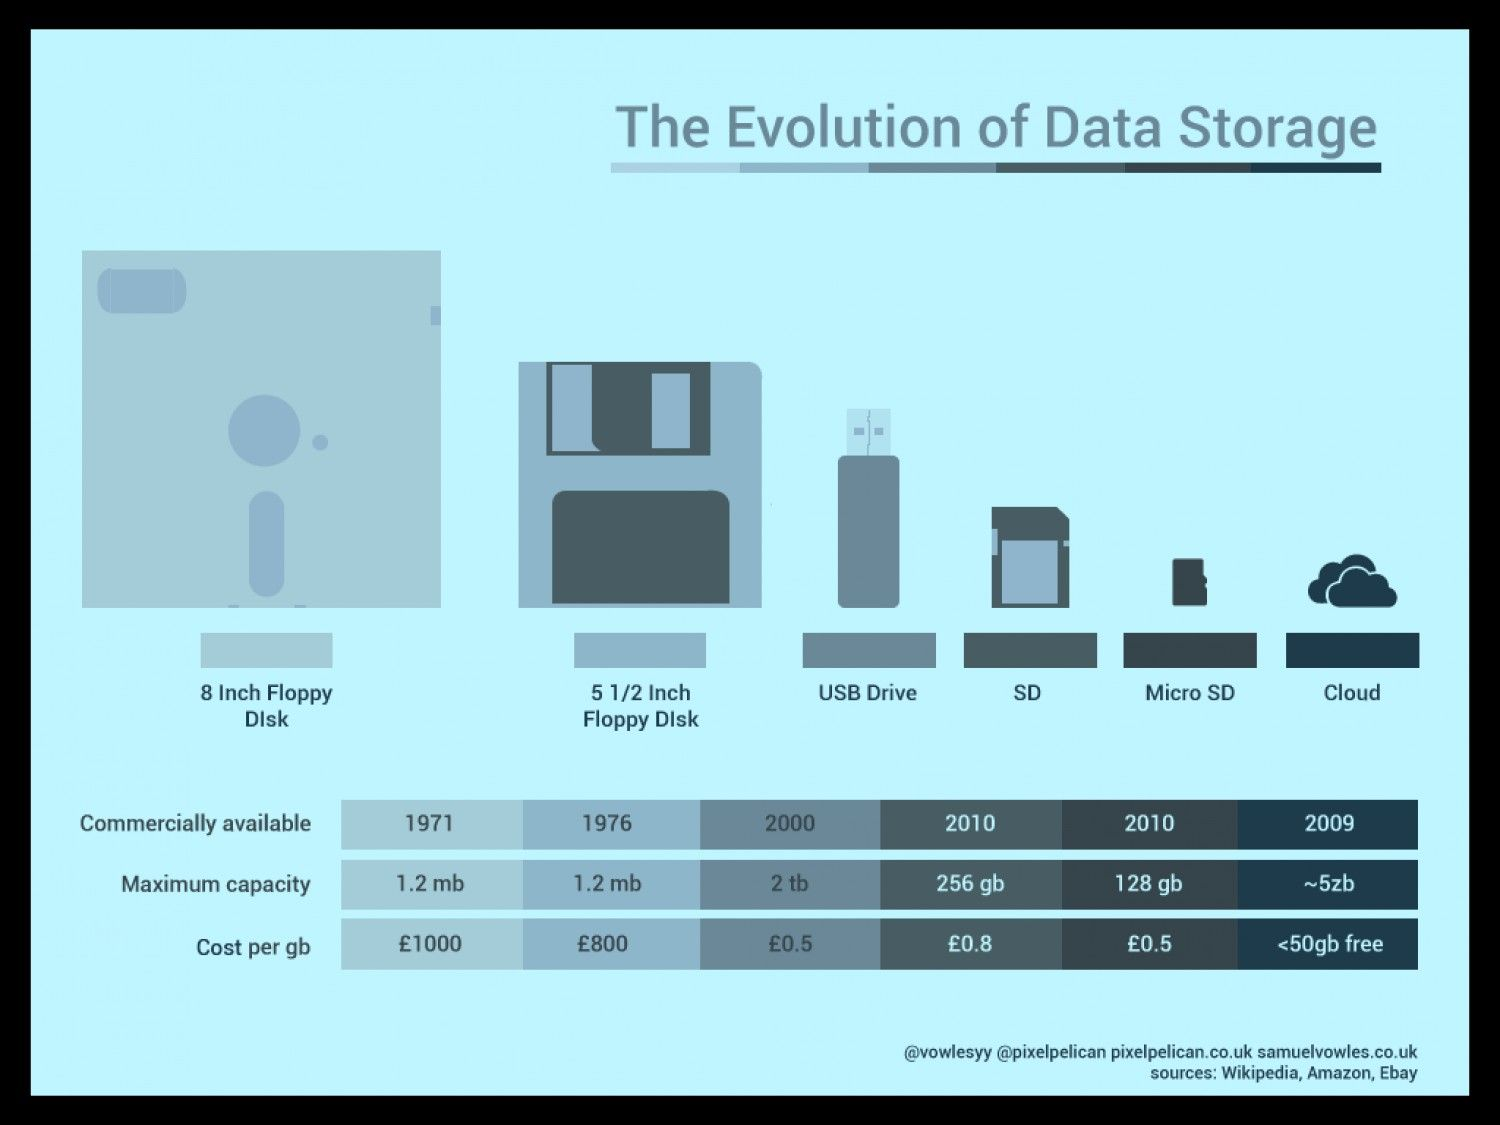
\includegraphics[width=.65\linewidth]{pictures/disk-evo.jpg}
    \caption{Evolución del espacio de almacenamiento en términos económicos y cuantitativos \cite{wecomputingtechStorageDevicesLondon}.}
    \label{fig:disk-evolution}
\end{figure}

Finalmente, el gran salto tecnológico se ha producido con la aparición de Internet y
las comunicaciones ya no eran únicamente personales sino entre dispositivos. En relación
con el punto anterior, la aparición de Internet ha permitido descentralizar el espacio
donde ya el usuario no guarda su información en su equipo personal sino en un clúster
de servidores distribuidos a nivel mundial al cual accede, de forma simultánea,
desde Internet y desde cualquier dispositivo. Así, lo que comenzó como una red de
conexión de unos pocos usuarios ha acabado convirtiéndose en la red global que
todos usamos y que conecta más de 4 billones de dispositivos (figura \ref{fig:internet-evo}).

\begin{figure}[H]
    \centering
    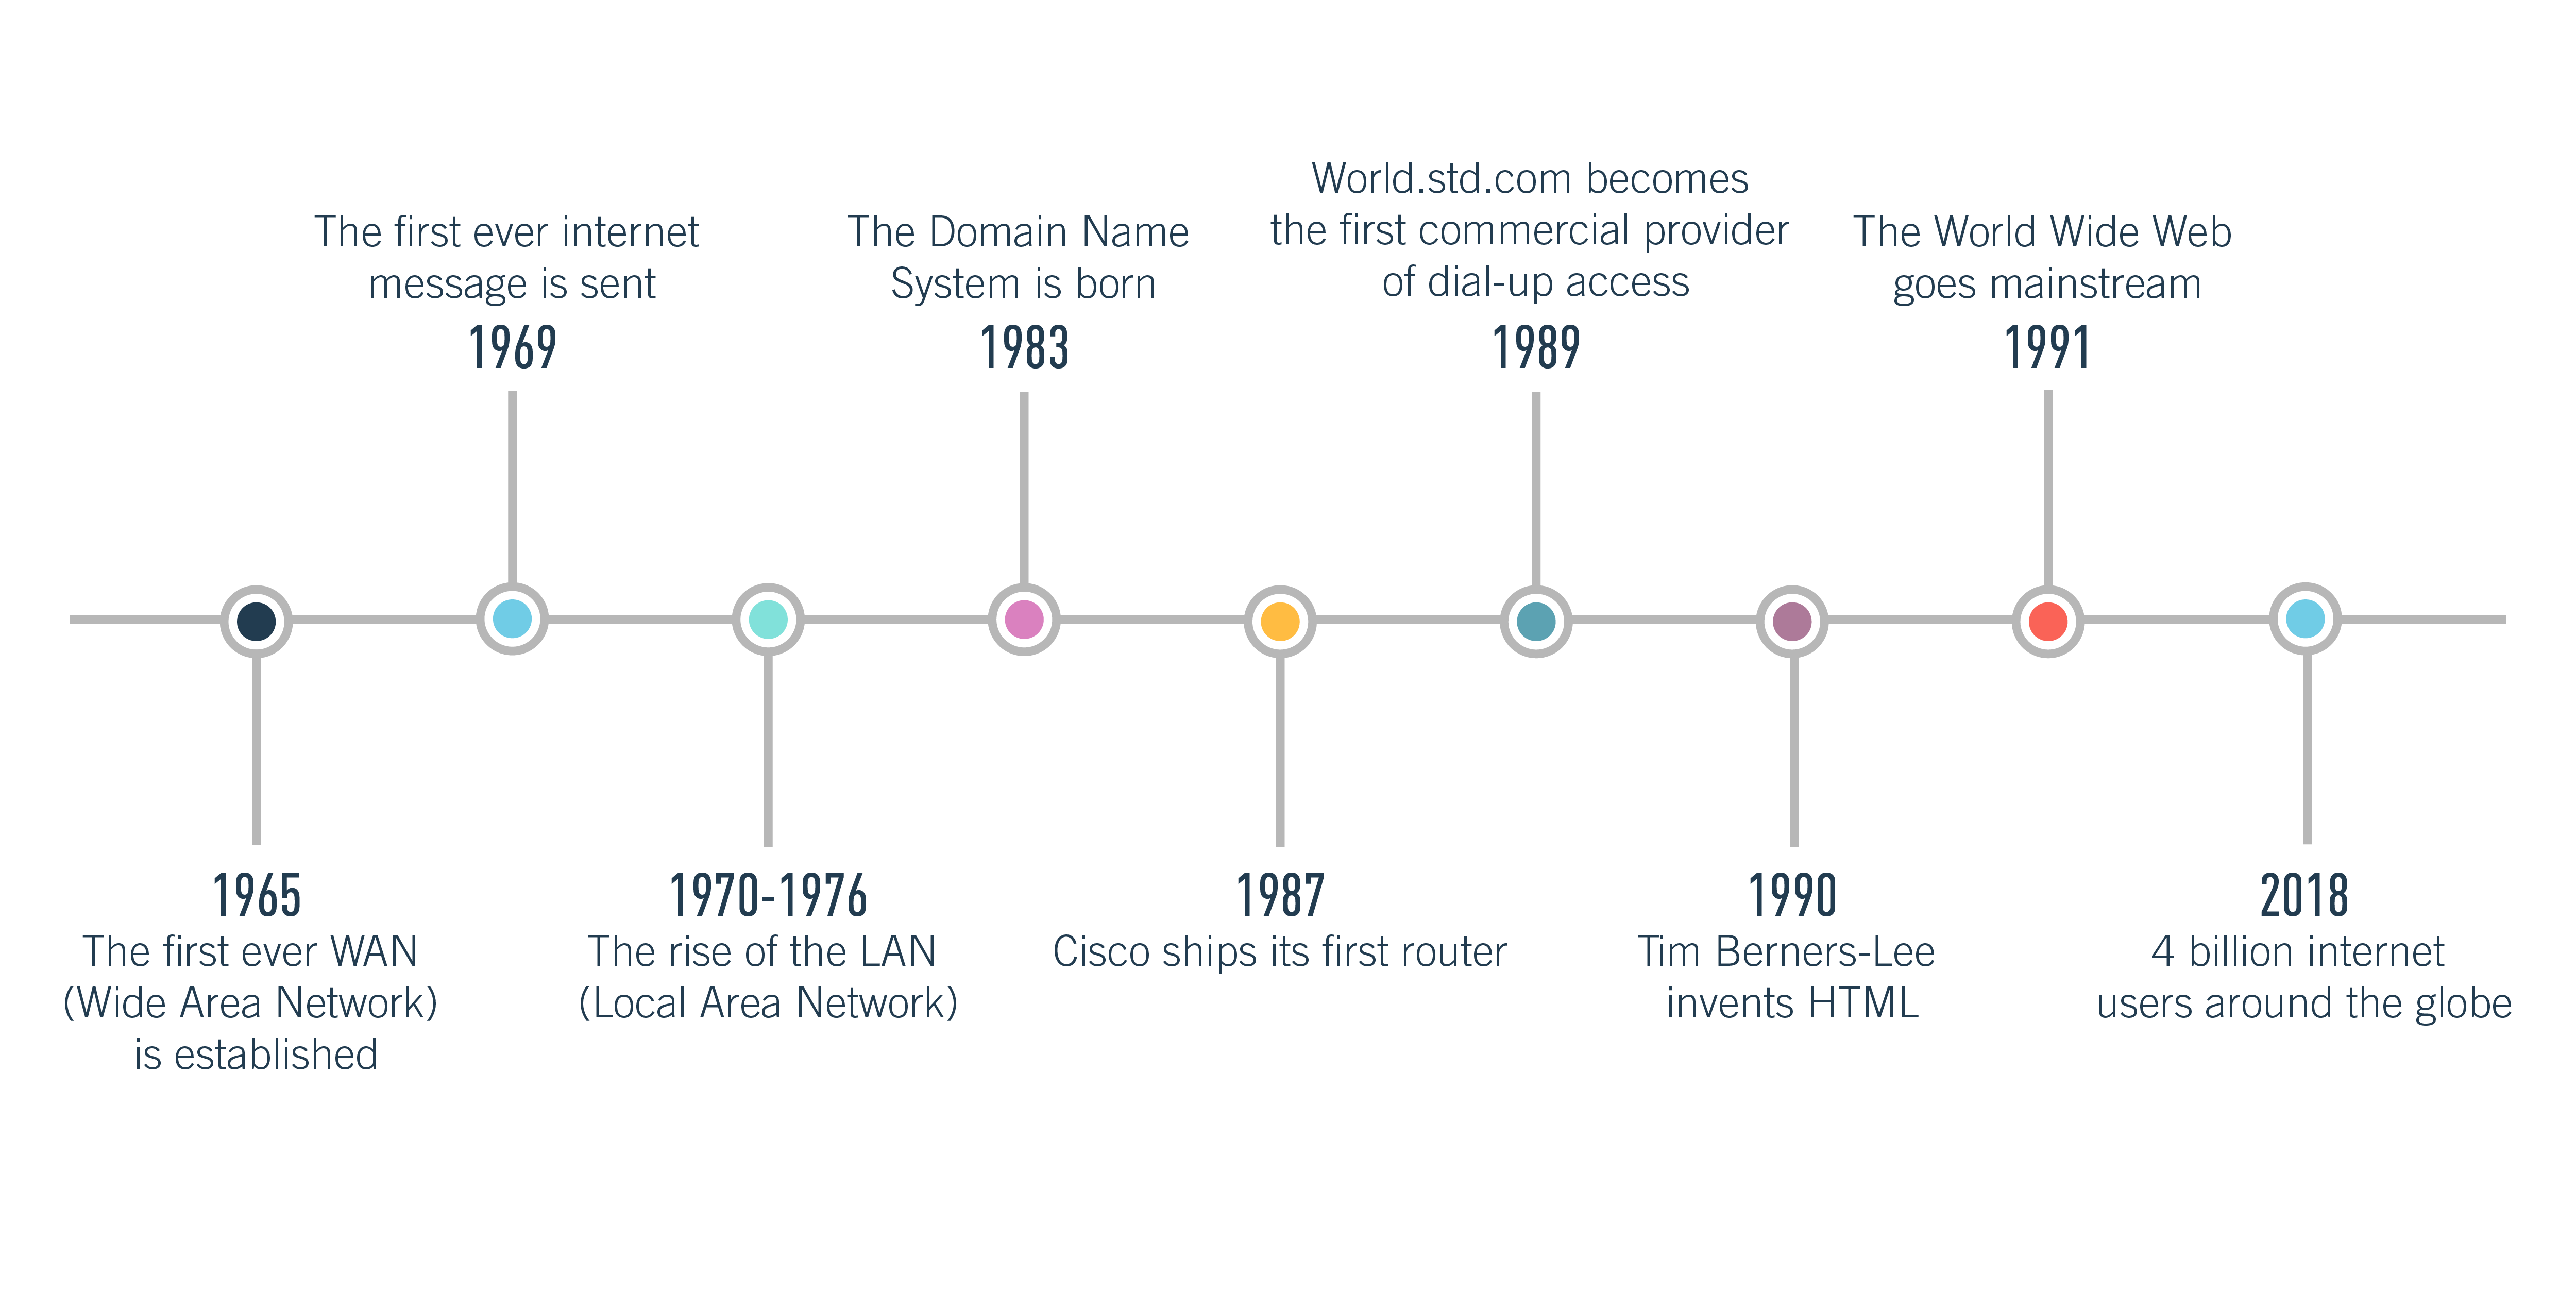
\includegraphics[width=.9\linewidth]{pictures/internet-timeline.png}
    \caption{Evolución de Internet a lo largo del tiempo, hasta llegar a hoy \cite{HowBecomeWeb}.}
    \label{fig:internet-evo}
\end{figure}

El problema a esto es evidente: con una mayor capacidad de cómputo, con más opciones
de comunicación y con más posibilidad de almacenar datos, los requisitos de las
aplicaciones van creciendo y creciendo y cada vez son más complejos de satisfacer,
no necesariamente a nivel \textit{hardware} (que por lo general suele acompañar)
sino a nivel \textit{software}. Como las aplicaciones se orientan a los usuarios
es necesario añadir capas de abstracción (como el sistema operativo) para facilitar
la labor a la persona. Sin embargo, cada capa nueva que se añade dificulta las tareas
de despliegue y mantenimiento dado que existe una gran variedad de combinaciones
\textit{hardware} y cada una puede estar con un sistema operativo distinto.

Por otra parte, la extensión de dependencias y posible incompatibilidad entre ellas
suele desembocar en el uso de versiones desactualizadas de una librería ya que tendríamos
``paquetes rotos''. Esto es tan común que tiene hasta su propio
término coloquial ``\textit{dependency hell}'' \cite{DependencyHell2021}. Contar con
dependencias obsoletas que ya han cumplido con su ciclo de vida \textit{software}
conlleva unas implicaciones de seguridad bastante severas:

\begin{itemize}
    \item Si un \textit{software} no ha mejorado a lo largo del tiempo, existe una
          malicia humana que puede aprovecharse de distintos \textit{exploits}
          existentes y comprometan nuestra aplicación.
    \item Un \textit{software} no actualizado puede tener implicaciones directas
          sobre el sistema en que se ejecuta, pudiendo producir fallos en el mismo.
          Esto se debe principalmente a que el \textit{hardware} sigue mejorando y
          creciendo y un \textit{software} antiguo puede presentar \textit{bugs}
          en dispositivos modernos que no presentaría en antiguos.
    \item Un \textit{software} no actualizado puede comprometer otros elementos del
          sistema en que se ejecuta. Por ejemplo, una aplicación `A' hace uso de dicho \textit{software}
          y una aplicación `B' también. Sin embargo, la última aplicación se ha diseñado
          para trabajar con la última versión del \textit{software} pero la aplicación
          `A' solo puede funcionar con una versión antigua e insegura. Por consiguiente,
          pese a que la aplicación `B' funcionaría correctamente el hecho de usar una
          versión antigua e insegura del \textit{software} compromete directamente al
          sistema y a la aplicación.
\end{itemize}

Es por eso que existen alternativas como ``\texttt{chroot}'' y máquinas virtuales para
subsanar estos problemas. Sin embargo, en los últimos años ha aparecido una herramienta
muy sonada y con gran éxito: Docker y los contenedores.
\subsection{¿Qué es Docker?}
\subsection{\textit{Real--life usages}}
\subsection{\textit{Docker rules}}

\section{Docker}
\subsection{Estructura de un Docker}
\subsection{Creación de un contenedor}
\subsection{Comunicación entre contenedores}
\subsection{Despliegue de aplicaciones multi--contenedores. \texttt{docker-compose}}
\subsection{``Orquestación'' de contenedores}
\subsection{Líneas futuras de desarrollo e innovación}

\section{Seguridad en Docker}
\subsection{Análisis de la pila Docker}
\subsection{Diferencias fundamentales con \texttt{chroot}}
\subsection{Seguridad en las comunicaciones de red -- \textit{firewall}}
\subsection{Seguridad en las comunicaciones inter--contenedores}

\printbibliography[heading=bibintoc]

\appendix

\end{document}